% ---------------------------------------------------------------
\section{Corpus selection}
\label{sec:sources}

Corpus extraction starts with a list of eligible sources. We require each source to have three features: an OpenAlex source identifier for corpus extraction, evidence from one of our journal registries that the source 
publishes economics or business research, and relatively high OpenAlex source topic density to exclude cross-disciplinary journals and other edge cases.

The journal registries are as follows. Harzing's \textit{71st Edition of the Journal Quality List}~\cite[][JQL]{harzinga.-w.JournalQualityList2024} assembles
peer assessments of journal quality across business and economics
disciplines. Its scope is confined to Economics and Commerce so no
filtering is applied.
The \textit{ERA 2023 Submission Journal List}~\cite[][SJL]{australianresearchcouncilERA2023Submission2022} assigns up to three
Field of Research (FoR) codes to each entry. From the full list 
of 26,241 journals we retain those having all FoR codes falling within 
Division~35 (Commerce, Management, Tourism and
Services) or Division~38 (Economics). This applies to two-digit `division' codes and all four-digit `group' codes (3501--3509, 3801--3803, 3899).
After filtering, 1,602~journals remain.
\textit{Clarivate Web of Science Journal Citation Reports} ~\cite[][JCR]{clarivateanalyticsJournalCitationReports2026} assign each
journal a Web of Science category. We retain those in Economics, Management, Business, Transportation or Business, Finance. After filtering, 1,413~journals remain.

Every journal in JQL, SJL, and MJL has at least one ISSN, and may have several. These registry ISSNs are joined independently to the OpenAlex sources snapshot using its list of ISSNs as the matching key. Journal titles are examined to identify around 30 additional matches where the OpenAlex source does not have an ISSN. The list of OpenAlex sources that are matched is designated OAS\textsuperscript{*}. The long list OAS\textsuperscript{*} includes sources publishing works in disciplines beyond  economics and business. We use OpenAlex source-topic assignments to exclude sources having a minority of works in economics/business. A source has work-topic counts for up to five topics, each within a single sub-field, field, and domain. We accumulate the work-topic counts for OpenAlex Field~14 (Economics, Econometrics and Finance) and Field~20 (Business and Management) and define the work-topic density is the ratio of this count to the total topic count in the source. Sources are dropped if this ratio is below 50\%. The 1,659 surviving sources, labeled OAS, are used to extract the corpus. Matching outcomes are summarised in Table \ref{tab:source_matching}.

\begin{table}[htbp]
	\centering
	\caption{Registry source matches to OpenAlex source identifiers}
	\label{tab:source_matching}
	\begin{tabular}{p{6cm} rrrr}
		\toprule
		Register & Journals & Matched & Match rate & Unmatched \\
		\midrule
		JQL (Harzing's journal quality list) & 842 & 839 & 99.6\% & 3 \\
		MJL (Clarivate master journal list) & 1,413 & 1,392 & 98.5\% & 21 \\
		SJL (ERA submission journal list)& 1,602 & 1,388 & 86.6\% & 214 \\
		\midrule
		\multicolumn{5}{l}{Registries pairwise overlap} \\
		\multicolumn{5}{l}{MJL $\cap$ SJL \hfill 783 sources} \\
		\multicolumn{5}{l}{MJL $\cap$ JQL \hfill 566 sources} \\
		\multicolumn{5}{l}{SJL $\cap$ JQL \hfill 424 sources} \\
		\multicolumn{5}{l}{MJL $\cap$ SJL $\cap$ JQL \hfill 393 sources} \\
		\midrule
		\multicolumn{5}{l}{OpenAlex topic filtering} \\
	    \multicolumn{5}{l}{MJL $\cap$ SJL $\cap$ JQL $\cap$ OA (OAS\textsuperscript{*} long-list) \hfill 2,380 sources} \\
 	    \multicolumn{5}{l}{OA sources with topics specifically in Economics or Commerce (OAS) \hfill 1,659 sources} \\
		\bottomrule
	\end{tabular}
\end{table}

We extract an initial corpus of works in the OAS source list, by retaining article and review types with publication years between 2020 and 2024 inclusive. We exclude works that are paratext or retract, or without an authorship entity. The institution retention curve Fig. \ref{fig:retention} implies that the preferred minimum cut for works per institution per year could be chosen as $\tau_U = 10$, leaving approximately 1,900 institutions and 75\% of the works. We will test values of $\tau_U = 5, 10\ \rm{and}\ 15$.

\begin{figure}[htbp]
	\centering
	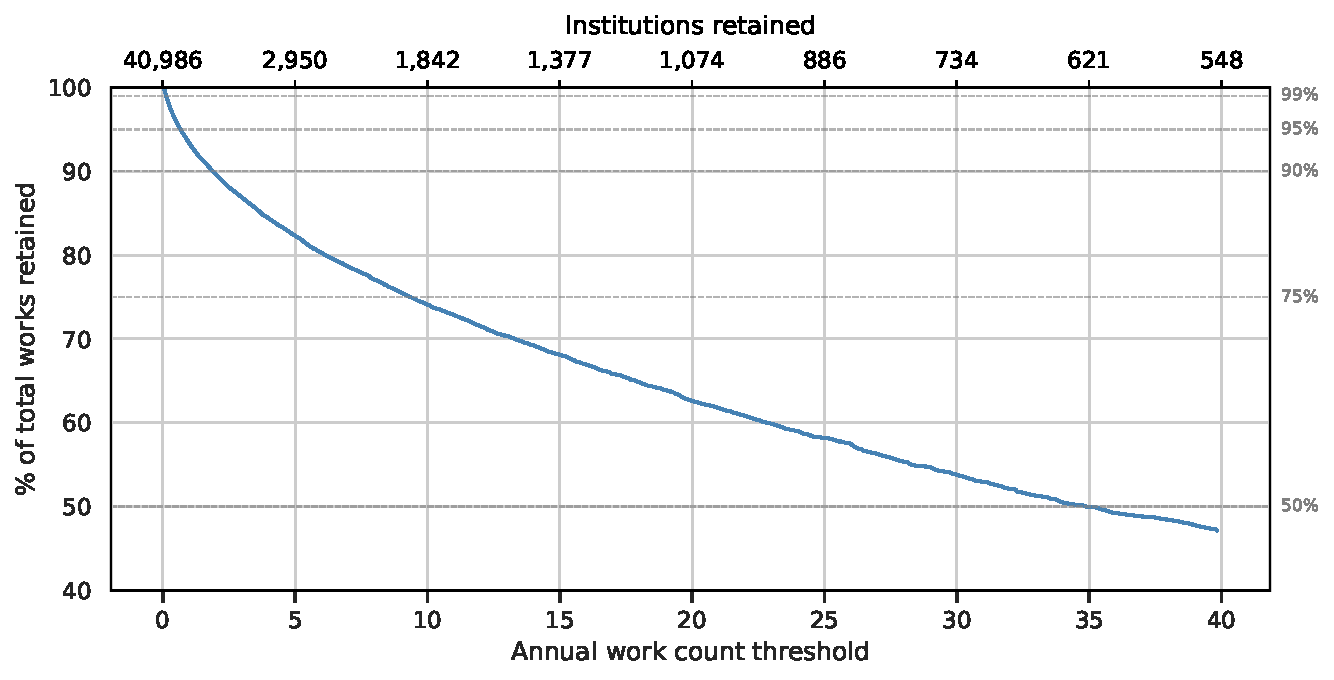
\includegraphics[width=0.8\textwidth]{../plots/plot1_institution_elbow_latex}
	\caption{Institution retention curve}
	\label{fig:retention}
\end{figure}
